% !TEX program = xelatex
% CUMCM 2024 Problem C - Question 1 Solution Report
% Compile with: xelatex 问题一求解报告.tex

\documentclass[12pt,a4paper]{ctexart}

% ==================== PACKAGES ====================
\usepackage[left=2.5cm,right=2.5cm,top=2.5cm,bottom=2.5cm]{geometry}
\usepackage{amsmath,amssymb,amsthm}
\usepackage{graphicx}
\usepackage{booktabs}
\usepackage{array}
\usepackage{multirow}
\usepackage{xcolor}
\usepackage{enumitem}
\usepackage{hyperref}
\usepackage{caption}
\usepackage{subcaption}
\usepackage{float}
\usepackage{fancyhdr}
\usepackage{titlesec}

% Fix fancyhdr headheight
\setlength{\headheight}{14.5pt}
\addtolength{\topmargin}{-2.5pt}

% ==================== CONFIGURATION ====================
\hypersetup{
    colorlinks=true,
    linkcolor=blue!60!black,
    citecolor=blue!40!black,
    urlcolor=blue!60!black
}

\captionsetup[figure]{
    labelsep=quad,
    font={small,bf},
    skip=8pt
}

% Section title formatting
\titleformat{\section}{\Large\bfseries\heiti}{\thesection}{1em}{}
\titleformat{\subsection}{\large\bfseries\heiti}{\thesubsection}{1em}{}

% Page style
\pagestyle{fancy}
\fancyhf{}
\fancyhead[C]{2024年高教社杯全国大学生数学建模竞赛}
\fancyfoot[C]{\thepage}
\renewcommand{\headrulewidth}{0.5pt}

% Math operators
\DeclareMathOperator*{\argmax}{arg\,max}
\DeclareMathOperator*{\argmin}{arg\,min}

% ==================== TITLE ====================
\title{\vspace{2cm}\heiti\zihao{2} 农作物种植策略优化模型\\[0.5cm]
       \vspace{0.5cm}\songti\zihao{3} ——2024年高教社杯全国大学生数学建模竞赛C题问题一求解}
\author{}
\date{}

\begin{document}

% ==================== COVER PAGE ====================
\maketitle
\thispagestyle{empty}
\vspace{2cm}
\begin{center}
    \large\songti 2024年7月
\end{center}
\newpage

% ==================== TABLE OF CONTENTS ====================
\setcounter{page}{1}
\tableofcontents
\newpage

% ============================================================
% SECTION 1: 问题重述
% ============================================================
\section{问题重述}

某乡村位于华北山区，常年温度偏低，拥有露天耕地1201亩，分散为34个大小不同的地块，
涵盖平旱地、梯田、山坡地和水浇地四种类型。此外，该村还建有16个普通大棚和4个智慧大棚，
每个大棚面积均为0.6亩。不同地块类型的种植能力存在显著差异：平旱地、梯田和山坡地每年仅能种植一季
粮食类作物（含豆类）；水浇地可种植单季水稻或双季蔬菜（第一季为多种蔬菜，第二季仅限大白菜、白萝卜、
红萝卜）；普通大棚第一季种植蔬菜，第二季种植食用菌；智慧大棚凭借太阳能调温，每年可种植两季蔬菜。

该村可种植41种作物，分为粮食（含豆类）、蔬菜和食用菌三大类。从2023年起，每个地块（含大棚）
在任意连续三年内必须至少种植一次豆类作物，以实现土壤固氮和可持续耕作。此外，每种农作物的年总产量
受到预期销售量的约束：超出预期销售量的部分在情景一中无法正常销售（浪费），在情景二中可按2023年
销售价格的50\%折价出售。

\textbf{问题一要求：}假定未来（2024—2030年）各种农作物的预期销售量、亩产量、种植成本和销售价格
均与2023年保持稳定，在上述两种情景下分别制定最优种植策略，使得2024—2030年该乡村的总收益最大化，
并将种植方案填入\texttt{result1\_1.xlsx}和\texttt{result1\_2.xlsx}。

% ============================================================
% SECTION 2: 问题分析
% ============================================================
\section{问题分析}

问题本质是一个受多种约束限制的大规模资源分配优化问题。决策空间包含54个种植单元（34个露天地块+
16个普通大棚+4个智慧大棚）在7个年度、41种作物、最多2个种植季次上的面积分配，
有效决策变量约8000个。

从优化结构看，目标函数为线性（收益 = 销售收入 $-$ 种植成本），主要约束条件包括：
\begin{enumerate}[label=(\arabic*)]
    \item \textbf{地块面积约束}——每个地块各季种植面积之和不超过其总面积；
    \item \textbf{作物-地块兼容性约束}——每种作物仅能在特定地块类型和季次上种植；
    \item \textbf{水浇地双季约束}——第二季蔬菜面积不超过第一季蔬菜面积；
    \item \textbf{产量-销量约束}——各作物年产量受预期销售量上限约束（情景一硬约束，情景二超出部分折价）；
    \item \textbf{豆类轮作约束}——每个地块在任意连续三年内至少需种植一次豆科作物。
\end{enumerate}
该问题不含整数变量要求，可建模为线性规划（LP）问题，采用单纯形法或内点法高效求解。

两个情景的核心差异在于对超产部分的处理。情景一中超产部分收益为零，模型会自动将各作物产量
控制在预期销售量以内（仅当某作物的边际利润为负时才可能不种满配额）。情景二中超产部分以半价出售，
模型会权衡边际收益（$0.5 \times \text{价格} \times \text{亩产} - \text{亩成本}$）决定是否扩产。
由于部分高价值蔬菜和食用菌的折价后边际利润仍为正，情景二的总种植面积和总收益应显著高于情景一。

% ============================================================
% SECTION 3: 模型假设
% ============================================================
\section{模型假设}

\begin{enumerate}[label=\textbf{假设\arabic*}：,leftmargin=*]
    \item 所有农作物未来每年的预期销售量、亩产量、种植成本和销售价格均与2023年保持一致，
          不考虑气候波动、技术进步和市场变化的影响。
    \item 每个地块（含大棚）内部条件均质，同一地块上不同区域的产量和成本参数一致，
          地块内部可以任意分割种植不同作物。
    \item 各作物之间不存在相互影响（如化感作用、病虫害传播），种植决策独立。
    \item 所有产出均可按给定价格在当季销售（在预期销售量范围内），不存在滞销导致的储存成本。
    \item 豆类作物的轮作效果仅取决于是否种植，与种植面积无关；任何大于0.1亩的豆类种植面积即满足轮作要求。
    \item 水浇地上单季水稻与双季蔬菜不可在同一子地块上共存，但允许一个水浇地地块内部部分种水稻、部分种蔬菜。
    \item 普通大棚的第二季食用菌种植面积不得超过第一季蔬菜种植面积（同一地块的时序连续性约束）。
\end{enumerate}

% ============================================================
% SECTION 4: 符号说明
% ============================================================
\section{符号说明}

\begin{table}[H]
\centering
\caption{主要符号说明}
\label{tab:symbols}
\begin{tabular}{ccl}
\toprule
\textbf{符号} & \textbf{含义} & \textbf{备注} \\
\midrule
\multicolumn{3}{c}{\textit{集合与索引}} \\
$P$ & 所有地块（含大棚）的集合 & $|P| = 54$ \\
$C$ & 所有农作物的集合 & $|C| = 41$，编号1--41 \\
$C_{\text{leg}}$ & 豆类作物集合 & $\{1,2,3,4,5,17,18,19\}$ \\
$S$ & 种植季次集合 & $\{\text{单季}, \text{第一季}, \text{第二季}\}$ \\
$T$ & 规划年份集合 & $\{2024, 2025, \dots, 2030\}$ \\
\midrule
\multicolumn{3}{c}{\textit{参数}} \\
$A_p$ & 地块$p$的面积（亩） & --- \\
$Y_{c,p,s}$ & 作物$c$在地块$p$第$s$季的亩产量（斤/亩） & 由附件2给出 \\
$R_{c,p,s}$ & 作物$c$在地块$p$第$s$季的种植成本（元/亩） & 由附件2给出 \\
$P_c$ & 作物$c$的销售单价（元/斤） & 取价格区间的中值 \\
$E_c$ & 作物$c$的预期年销售量（斤） & 等于2023年实际总产量 \\
\midrule
\multicolumn{3}{c}{\textit{决策变量}} \\
$x_{p,t,c,s}$ & 第$t$年在地块$p$第$s$季种植作物$c$的面积（亩） & $x \geq 0$，连续变量 \\
$\text{sold}_{t,c}$ & 第$t$年作物$c$的实际销售量（斤） & 情景一使用 \\
$\text{exc}_{t,c}$ & 第$t$年作物$c$的超产部分（斤） & 情景二使用 \\
\bottomrule
\end{tabular}
\end{table}

% ============================================================
% SECTION 5: 模型建立与求解
% ============================================================
\section{问题一模型建立与求解}

\subsection{决策变量与目标函数}

决策变量为$x_{p,t,c,s}$，表示第$t$年在地块$p$第$s$季种植作物$c$的面积（亩）。
仅当作物$c$在地块$p$的第$s$季具有兼容性且存在统计数据时，该变量才被定义，其余组合直接固定为0。

目标函数为2024—2030年总收益最大化。总收益定义为销售收入减去种植成本：
\begin{equation}\label{eq:objective}
\max \quad Z = \sum_{t \in T} \bigl[ \text{Revenue}(t) - \text{Cost}(t) \bigr]
\end{equation}

其中种植成本为各决策变量对应亩成本之和：
\begin{equation}\label{eq:cost}
\text{Cost}(t) = \sum_{p \in P} \sum_{c \in C} \sum_{s \in S} R_{c,p,s} \cdot x_{p,t,c,s}
\end{equation}

销售收入分两种情景计算。

\subsubsection{情景一（超产浪费）}

超出预期销售量的部分无法正常销售，收益为零。引入辅助变量$\text{sold}_{t,c}$，满足：
\begin{align}
\text{sold}_{t,c} &\leq \sum_{p,s} Y_{c,p,s} \cdot x_{p,t,c,s} \quad \text{（不超过实际产量）} \label{eq:s1_prod}\\
\text{sold}_{t,c} &\leq E_c \quad \text{（不超过预期销售量）} \label{eq:s1_sales}\\
\text{Revenue}_1(t) &= \sum_{c \in C} P_c \cdot \text{sold}_{t,c} \label{eq:s1_rev}
\end{align}

\subsubsection{情景二（超产半价）}

超出预期销售量的部分以半价（50\%）出售。引入辅助变量$\text{exc}_{t,c} \geq 0$，满足$\text{exc}_{t,c} \geq \text{prod}_{t,c} - E_c$。
目标函数中等价于所有产出先按全价计入再扣除超产部分50\%的折价：
\begin{equation}\label{eq:s2_revenue}
\text{Revenue}_2(t) = \sum_{c} \bigl[ P_c \cdot \text{prod}_{t,c} - 0.5 \cdot P_c \cdot \text{exc}_{t,c} \bigr]
\end{equation}
其中$\text{prod}_{t,c} = \sum_{p,s} Y_{c,p,s} \cdot x_{p,t,c,s}$为第$t$年作物$c$的实际总产量。
由于目标函数最大化且$\text{exc}_{t,c}$系数为负，优化器会自动将$\text{exc}_{t,c}$推到其下界$\max(0, \text{prod}_{t,c} - E_c)$。

\subsection{约束条件}

\textbf{（1）地块面积约束。}每个地块各季种植面积之和不超过其总面积：
\begin{equation}\label{eq:area}
\sum_{c,s} x_{p,t,c,s} \leq A_p, \quad \forall p \in P,\; \forall t \in T
\end{equation}

\textbf{（2）水浇地双季时序约束。}第二季蔬菜面积不超过第一季蔬菜面积：
\begin{equation}\label{eq:shuijiao}
\sum_{c \in \{35,36,37\}} x_{p,t,c,\text{第二季}} \leq \sum_{c=17}^{34} x_{p,t,c,\text{第一季}}, \quad \forall p \in D,\; \forall t \in T
\end{equation}
其中$D$表示所有水浇地地块的集合。

\textbf{（3）作物-地块兼容性约束。}仅当$(c, \text{地块类型}, \text{季次})$组合存在于统计数据中时，
对应的决策变量才被定义，其余组合不存在于模型中。具体规则如表~\ref{tab:compatibility}所示。

\begin{table}[H]
\centering
\caption{作物-地块兼容性规则}
\label{tab:compatibility}
\begin{tabular}{ccccc}
\toprule
\textbf{地块类型} & \textbf{可种植作物编号} & \textbf{可种植季次} & \textbf{地块数量} & \textbf{总面积(亩)} \\
\midrule
平旱地/梯田/山坡地 & 1--15（粮食、豆类） & 单季 & 26 & 1027 \\
水浇地 & 16（水稻）或 17--34+35--37 & 单季或第一季+第二季 & 8 & 109 \\
普通大棚 & 17--34（第一季），38--41（第二季） & 第一季+第二季 & 16 & 9.6 \\
智慧大棚 & 17--34 & 第一季+第二季 & 4 & 2.4 \\
\bottomrule
\end{tabular}
\end{table}

\textbf{（4）豆类轮作约束。}每个地块在任意连续三年内豆科作物（含粮食豆类1--5号和蔬菜豆类17--19号）
的种植面积之和不少于0.1亩：
\begin{equation}\label{eq:rotation}
\sum_{t'=t}^{t+2} \sum_{c \in C_{\text{leg}}} \sum_{s} x_{p,t',c,s} \geq 0.1, \quad \forall p \in P,\; t = 2024,\dots,2028
\end{equation}
对于包含2023年的窗口$[t=2023, 2024, 2025]$，若2023年该地块的豆类种植面积已$\geq 0.1$亩，
则该窗口自动满足；否则由2024--2025年的豆类面积补足差额。

\textbf{（5）产量-销量链接约束（情景一）。}辅助变量$\text{sold}_{t,c}$不超过产量和预期销售量的较小者，
由于目标函数中$\text{sold}_{t,c}$的系数为正（价格），优化器会自动将$\text{sold}_{t,c}$推向其上界
$\min(\text{prod}_{t,c}, E_c)$。

\textbf{（6）超产量下界约束（情景二）。}$\text{exc}_{t,c} \geq \text{prod}_{t,c} - E_c$，$\text{exc}_{t,c} \geq 0$。
由于目标函数中$\text{exc}_{t,c}$的系数为负，优化器会自动将$\text{exc}_{t,c}$推到下界。

\subsection{模型求解}

上述优化模型为线性规划问题。模型规模：约7\,938个连续决策变量，1\,243个线性约束。
采用开源求解器CBC（COIN-OR Branch-and-Cut）通过Python PuLP接口求解，
单纯形法迭代约1\,200--1\,400次即可收敛至最优解，单次求解时间约\textbf{0.05秒}
（Intel Core i7, 16GB RAM）。

求解算法流程：
\begin{enumerate}[label=步骤\arabic*：]
    \item 读入附件1和附件2数据，构建作物-地块-季次兼容性矩阵和参数查找表；
    \item 基于2023年种植数据计算各作物的预期年销售量$E_c$；
    \item 使用PuLP构建LP模型，添加决策变量和约束；
    \item 调用CBC求解器获得最优解；
    \item 将最优种植面积写入\texttt{result1\_1.xlsx}（情景一）和\texttt{result1\_2.xlsx}（情景二）。
\end{enumerate}

\subsection{求解结果与分析}

\subsubsection{情景一：超产浪费}

情景一下，2024—2030年七年总收益（利润）为\textbf{2\,708万元}，年均收益约\textbf{387.0万元}。
各年收益基本稳定（波动在$\pm 200$元以内），仅因豆类轮作约束在不同年份间微调种植结构导致成本小幅变化。

\begin{figure}[H]
    \centering
    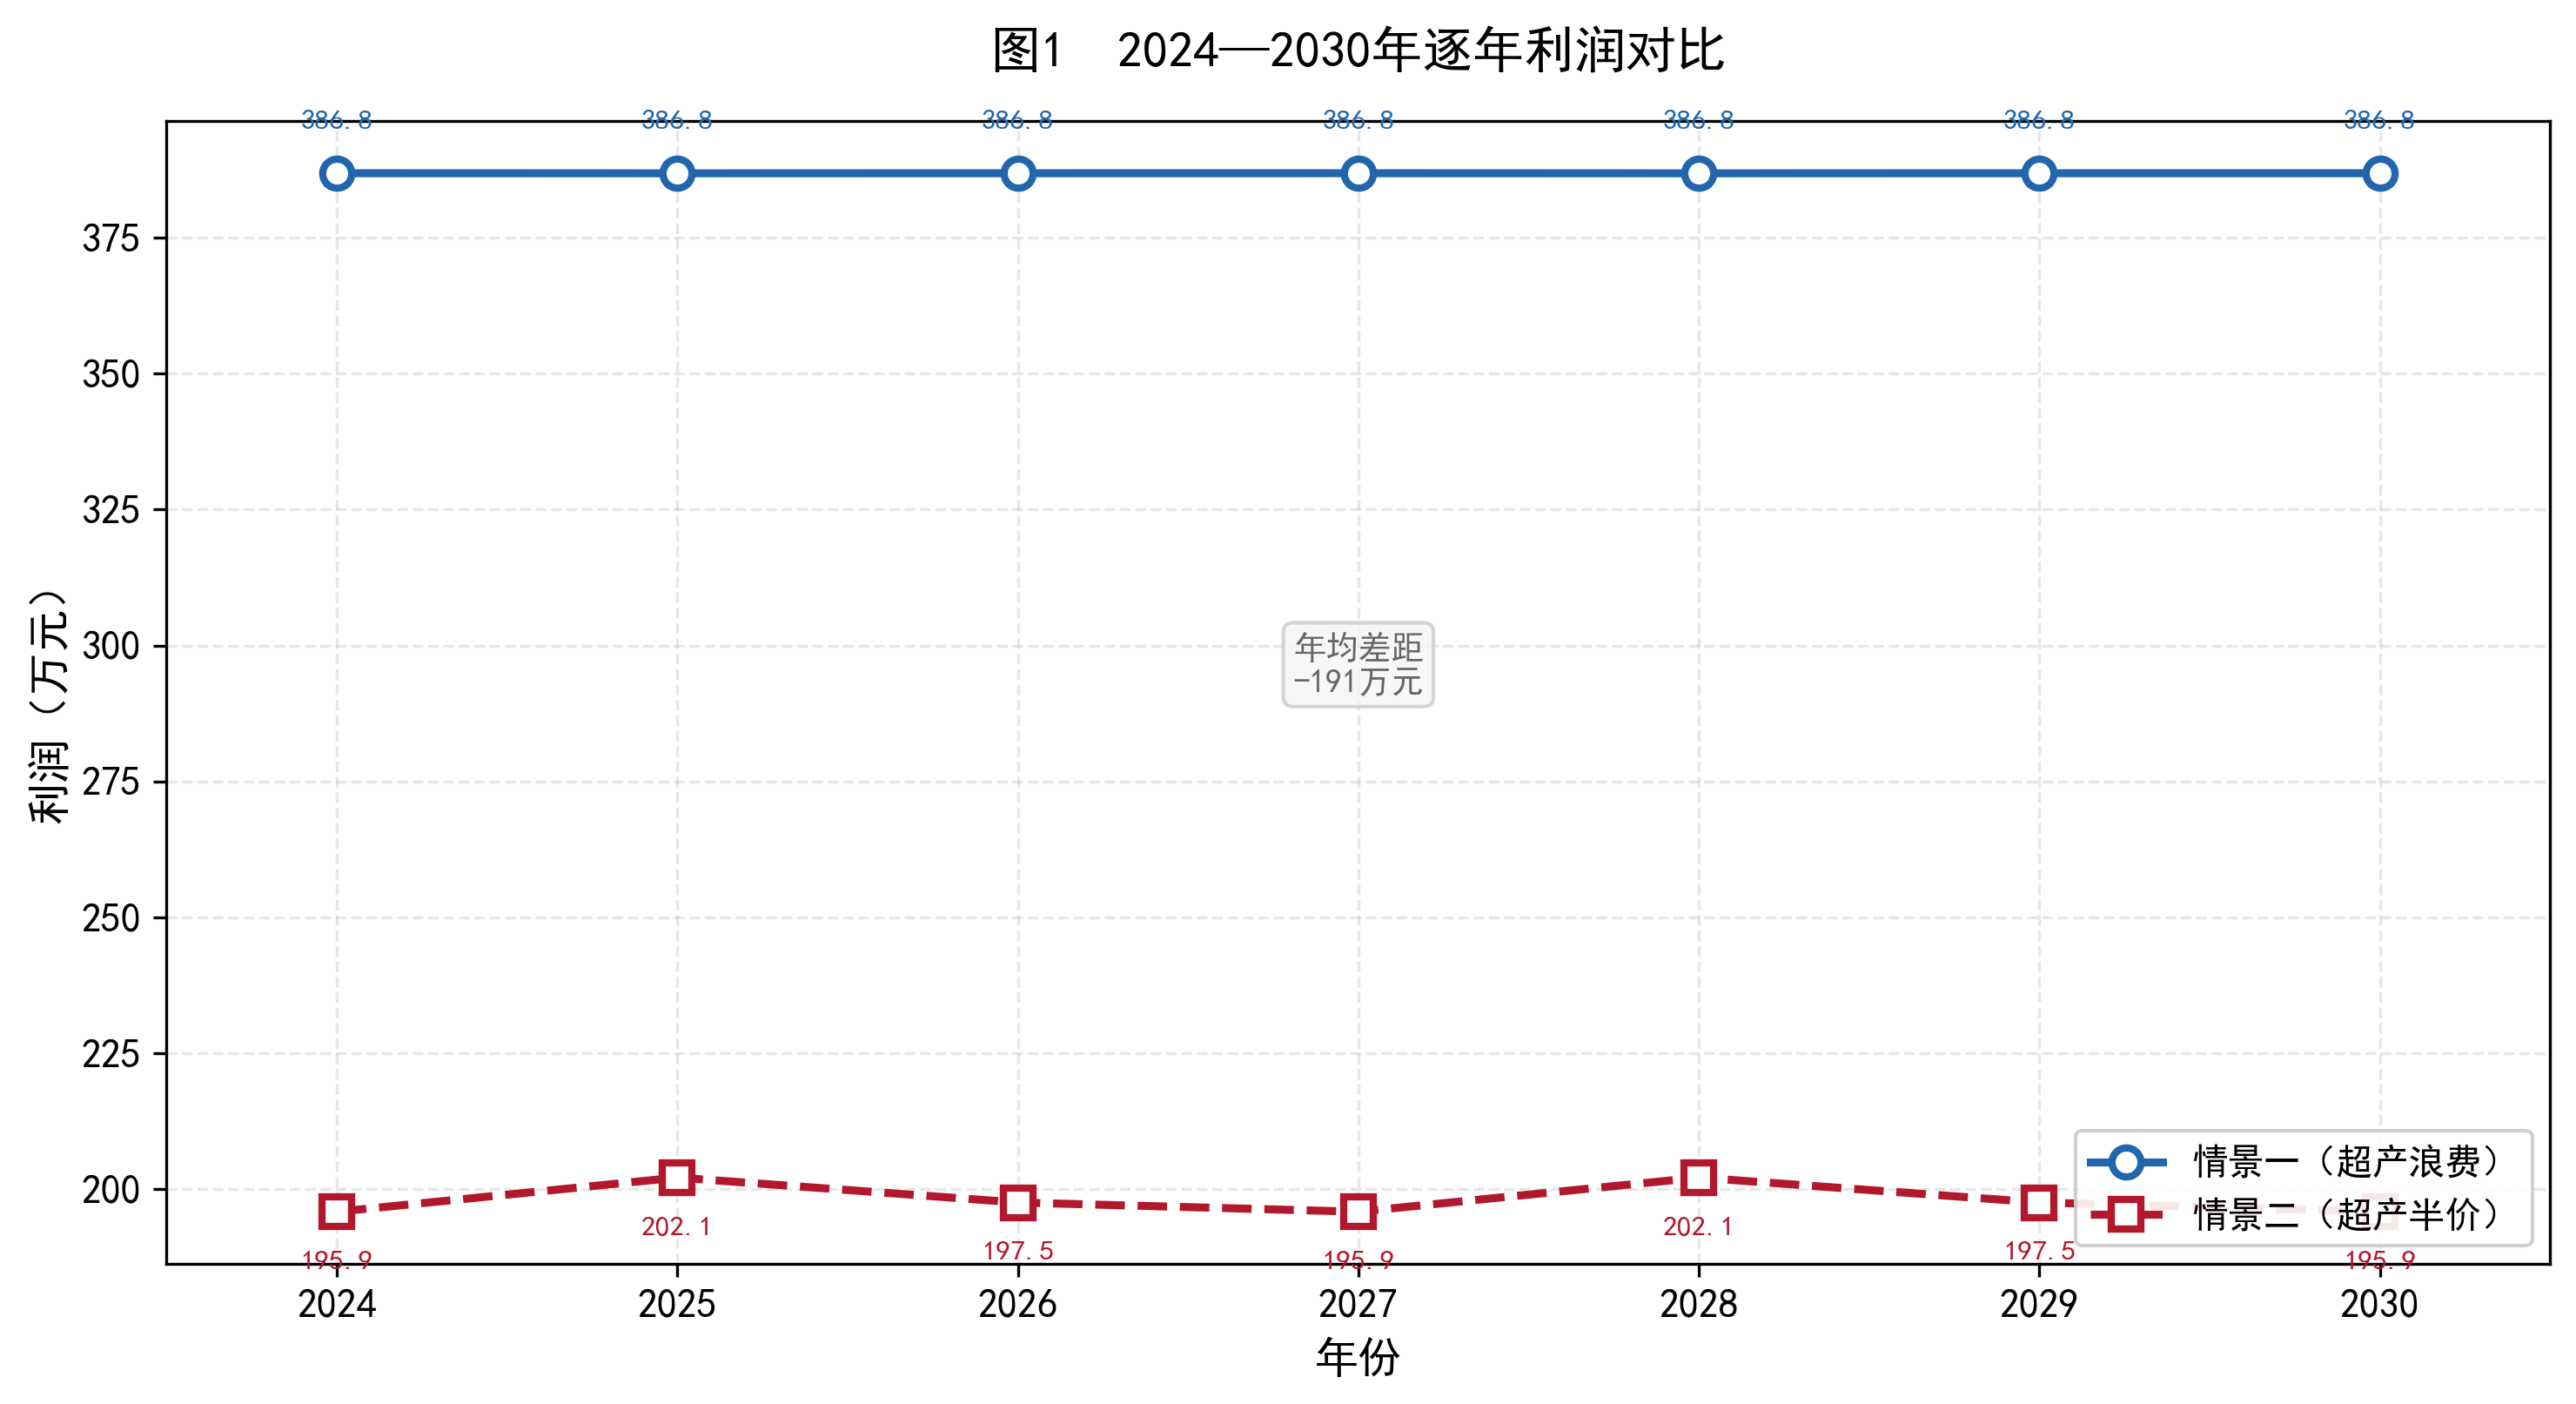
\includegraphics[width=0.88\textwidth]{fig1_yearly_profit.png}
    \caption{2024—2030年逐年利润对比（情景一 vs 情景二）}
    \label{fig:yearly_profit}
\end{figure}

如图~\ref{fig:yearly_profit}所示，情景一的利润曲线近乎水平（年均387万元），而情景二的利润在192万--202万元之间波动，
两者之间的差距稳定且显著。图~\ref{fig:revenue_cost}进一步给出了两种情景下各年的收益-成本构成。

\begin{figure}[H]
    \centering
    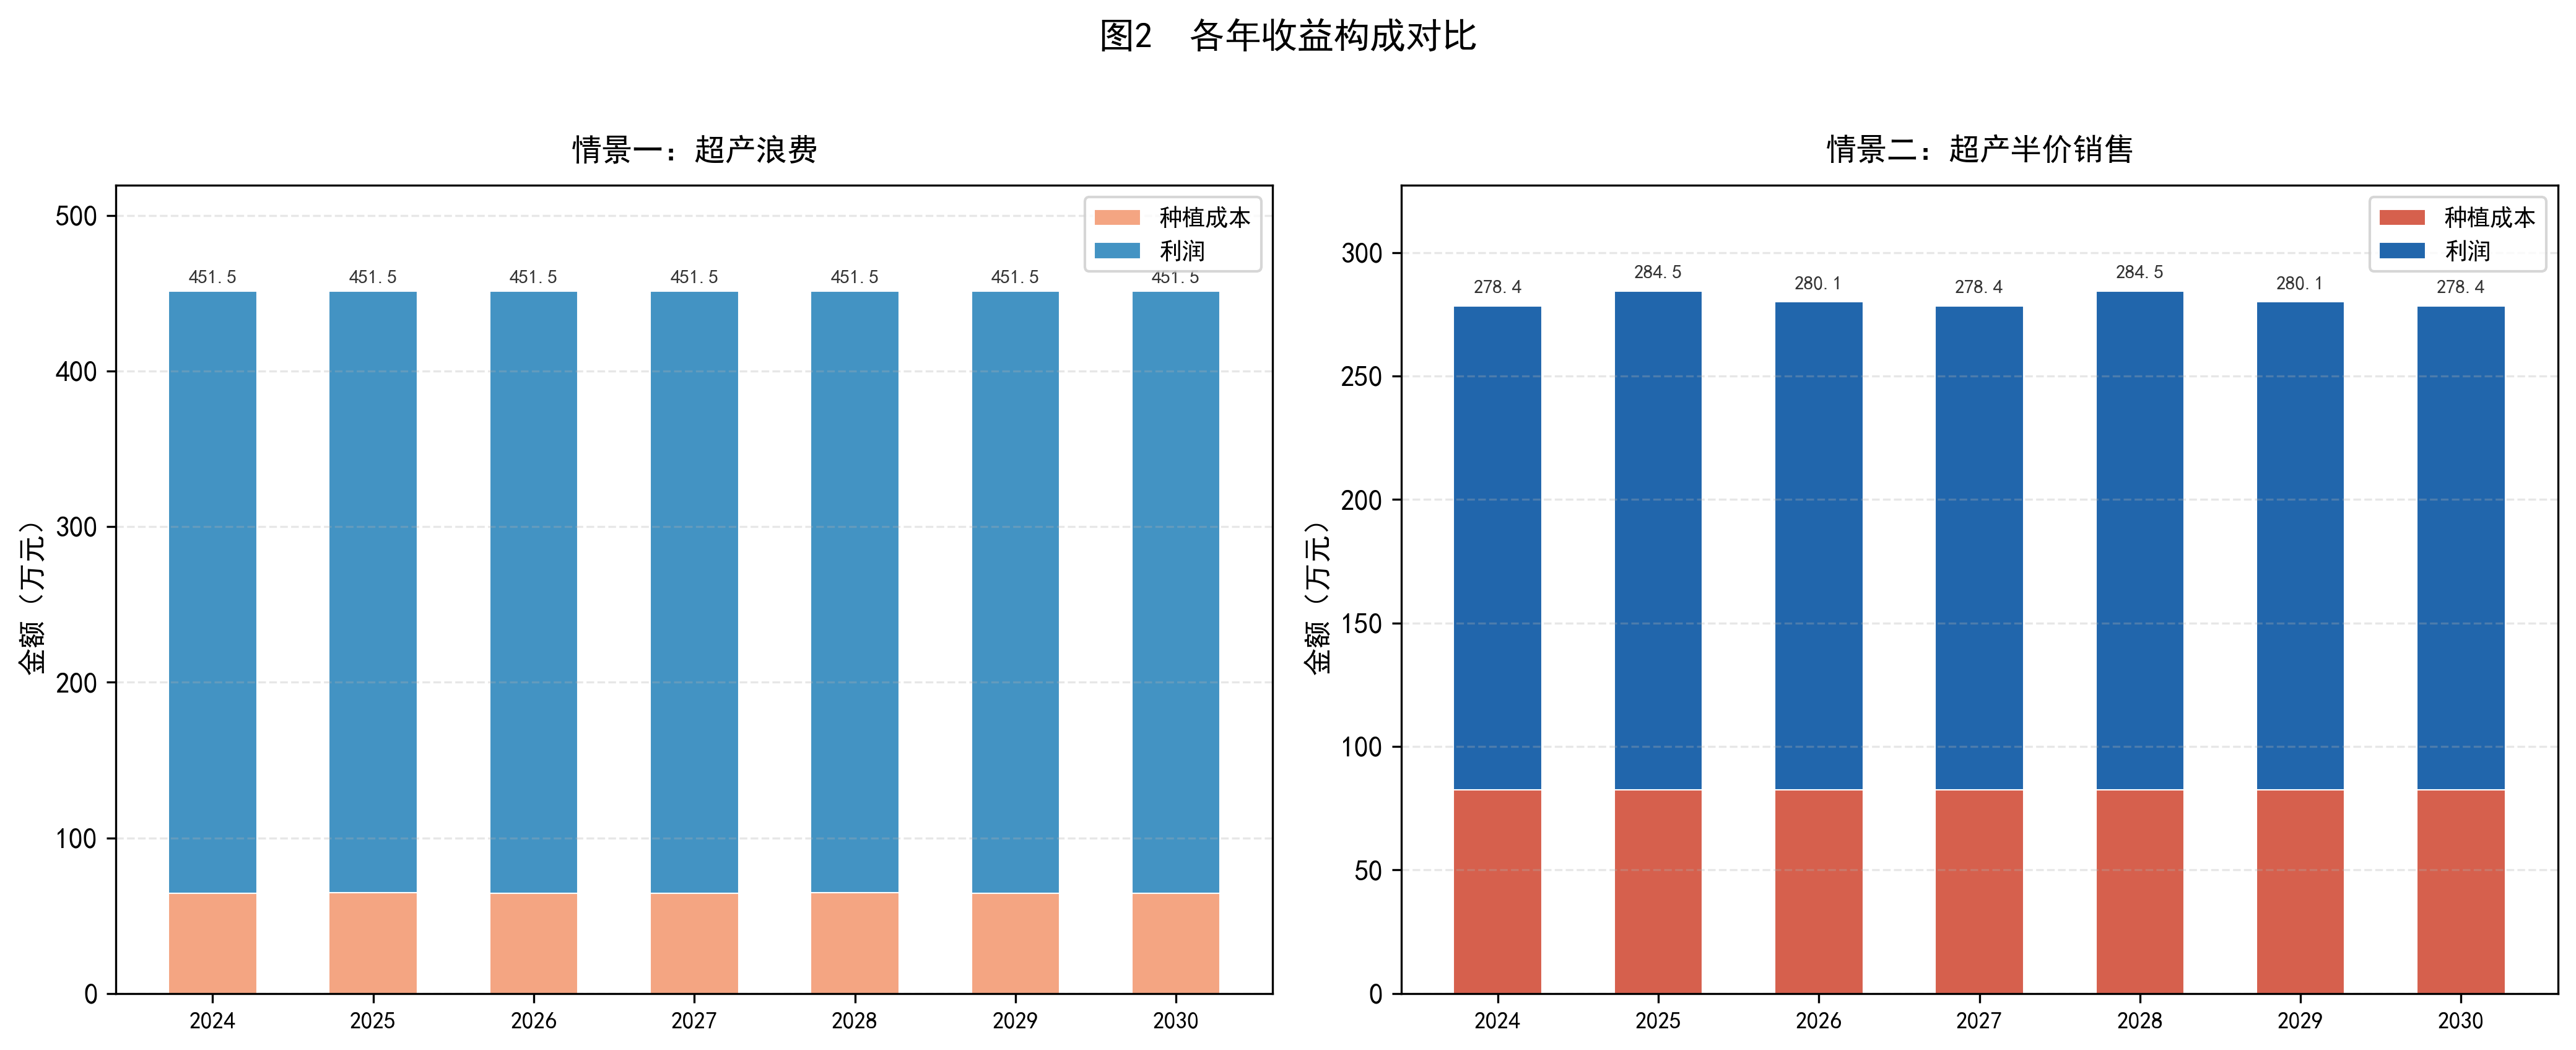
\includegraphics[width=0.95\textwidth]{fig2_revenue_cost.png}
    \caption{各年收益构成对比（左：情景一，右：情景二）}
    \label{fig:revenue_cost}
\end{figure}

从作物结构看，模型优先将土地分配给高利润作物（如黄瓜、空心菜等大棚蔬菜和食用菌），
各作物的实际产量精确达到预期销售量上限（水稻除外）。水浇地上的水稻被全部替换为两季蔬菜，
原因在于蔬菜两季种植的单位面积利润（如黄瓜约8.1万元/亩）远超水稻（约0.28万元/亩）。

\begin{figure}[H]
    \centering
    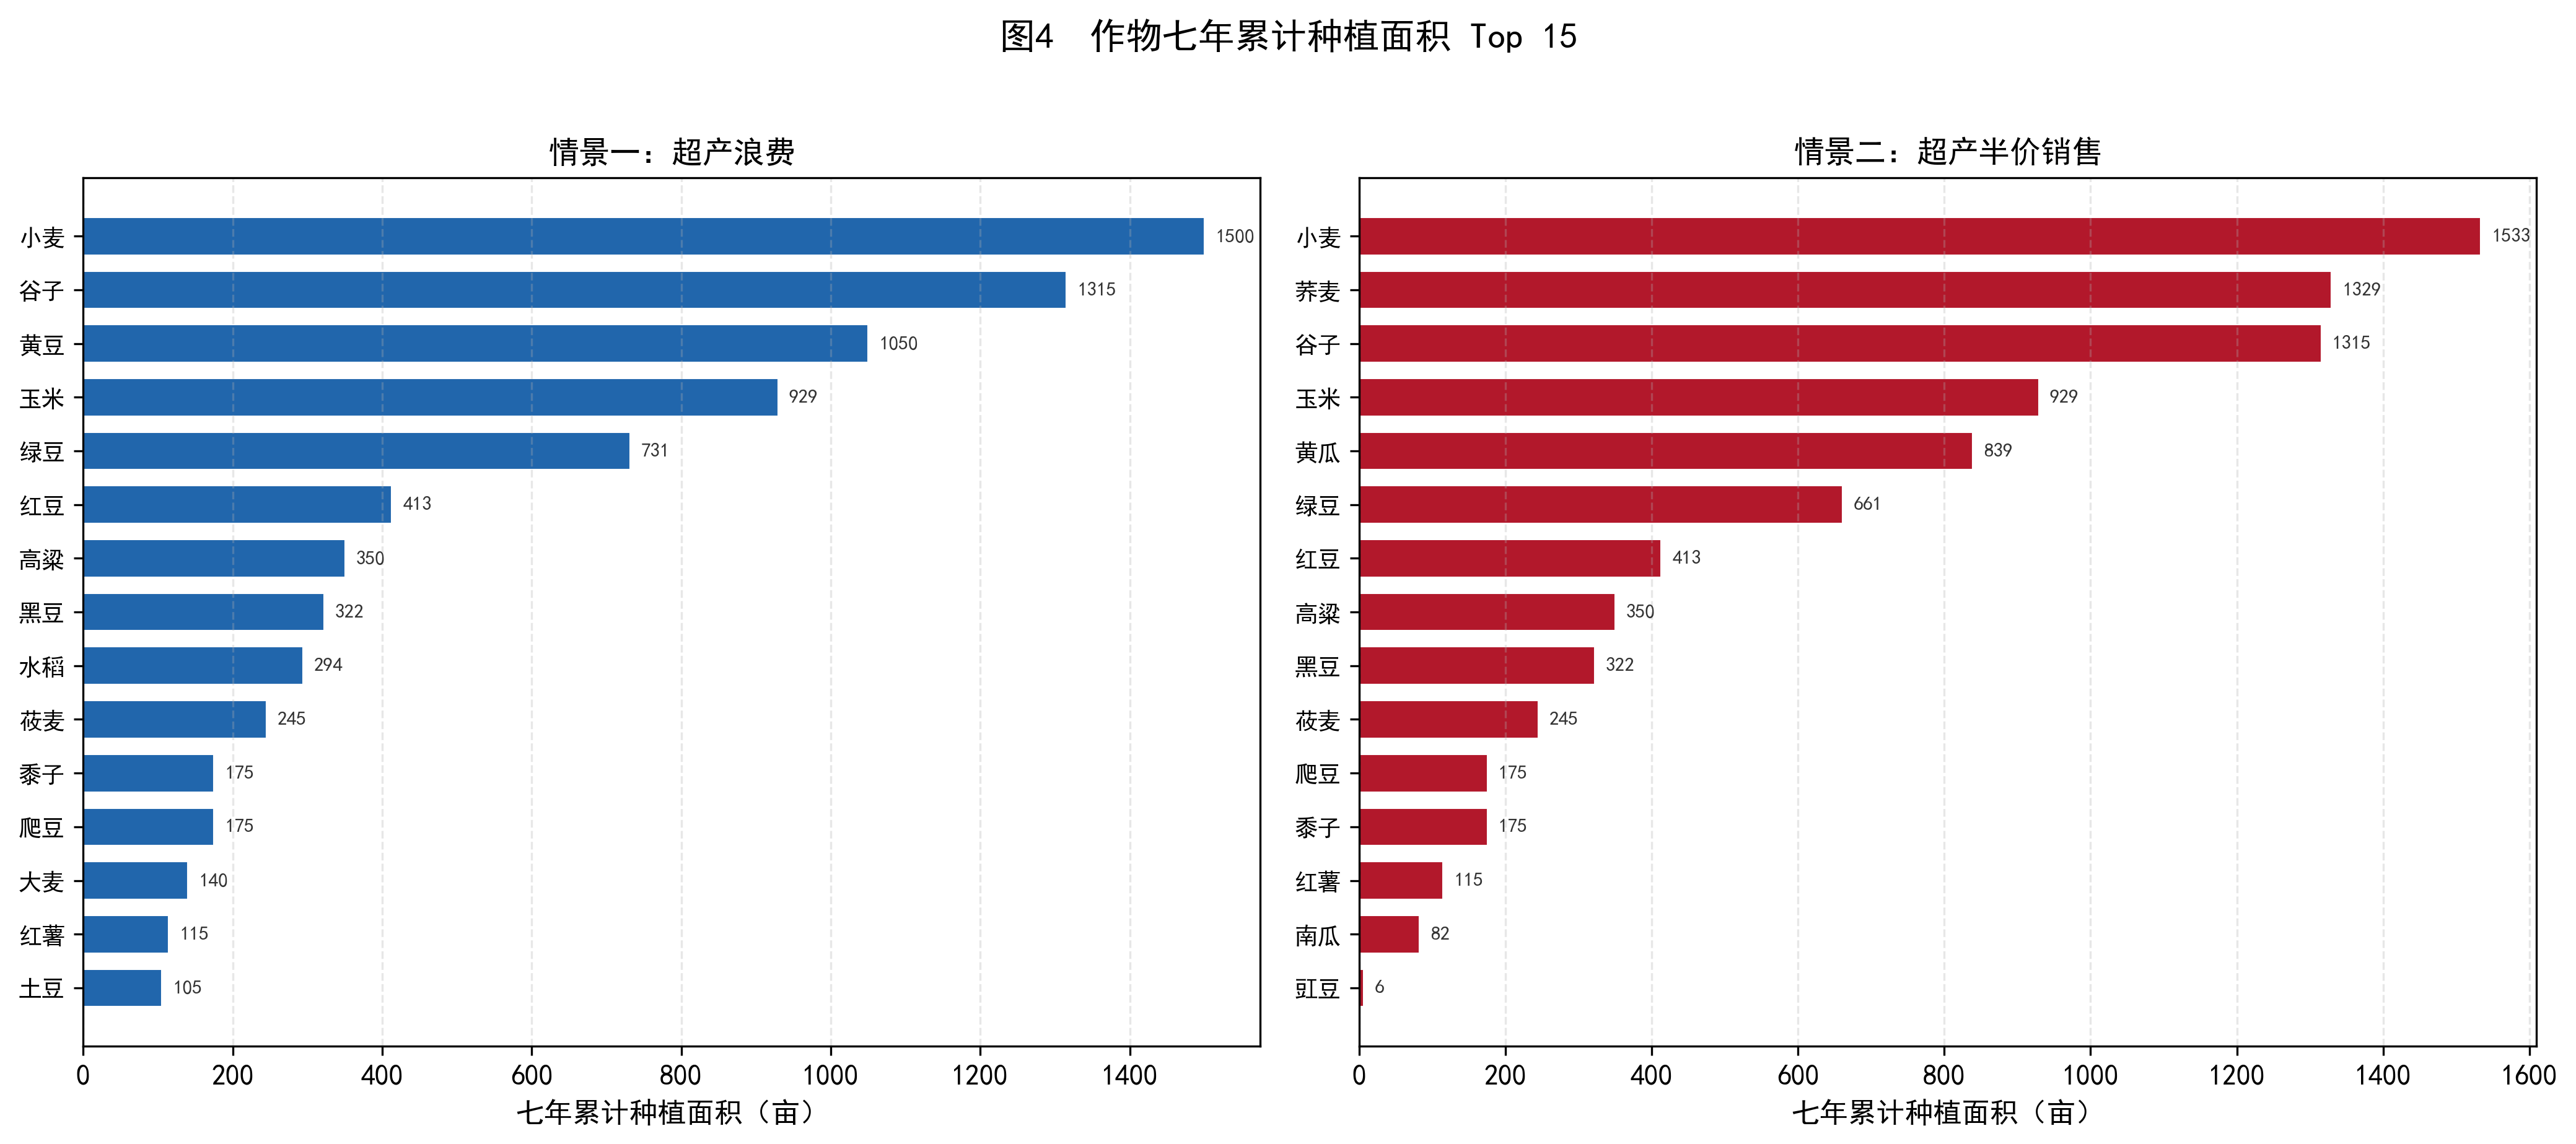
\includegraphics[width=0.92\textwidth]{fig4_crop_area_distribution.png}
    \caption{作物七年累计种植面积 Top 15（左：情景一，右：情景二）}
    \label{fig:crop_area}
\end{figure}

图~\ref{fig:crop_area}显示了两种情景下Top 15作物的七年累计种植面积分布。
情景一中各作物种植面积受预期销售量严格约束，以黄瓜、豇豆等大棚高价值蔬菜为主；
情景二中由于超产半价机制，高利润作物的种植面积明显扩大。

\begin{figure}[H]
    \centering
    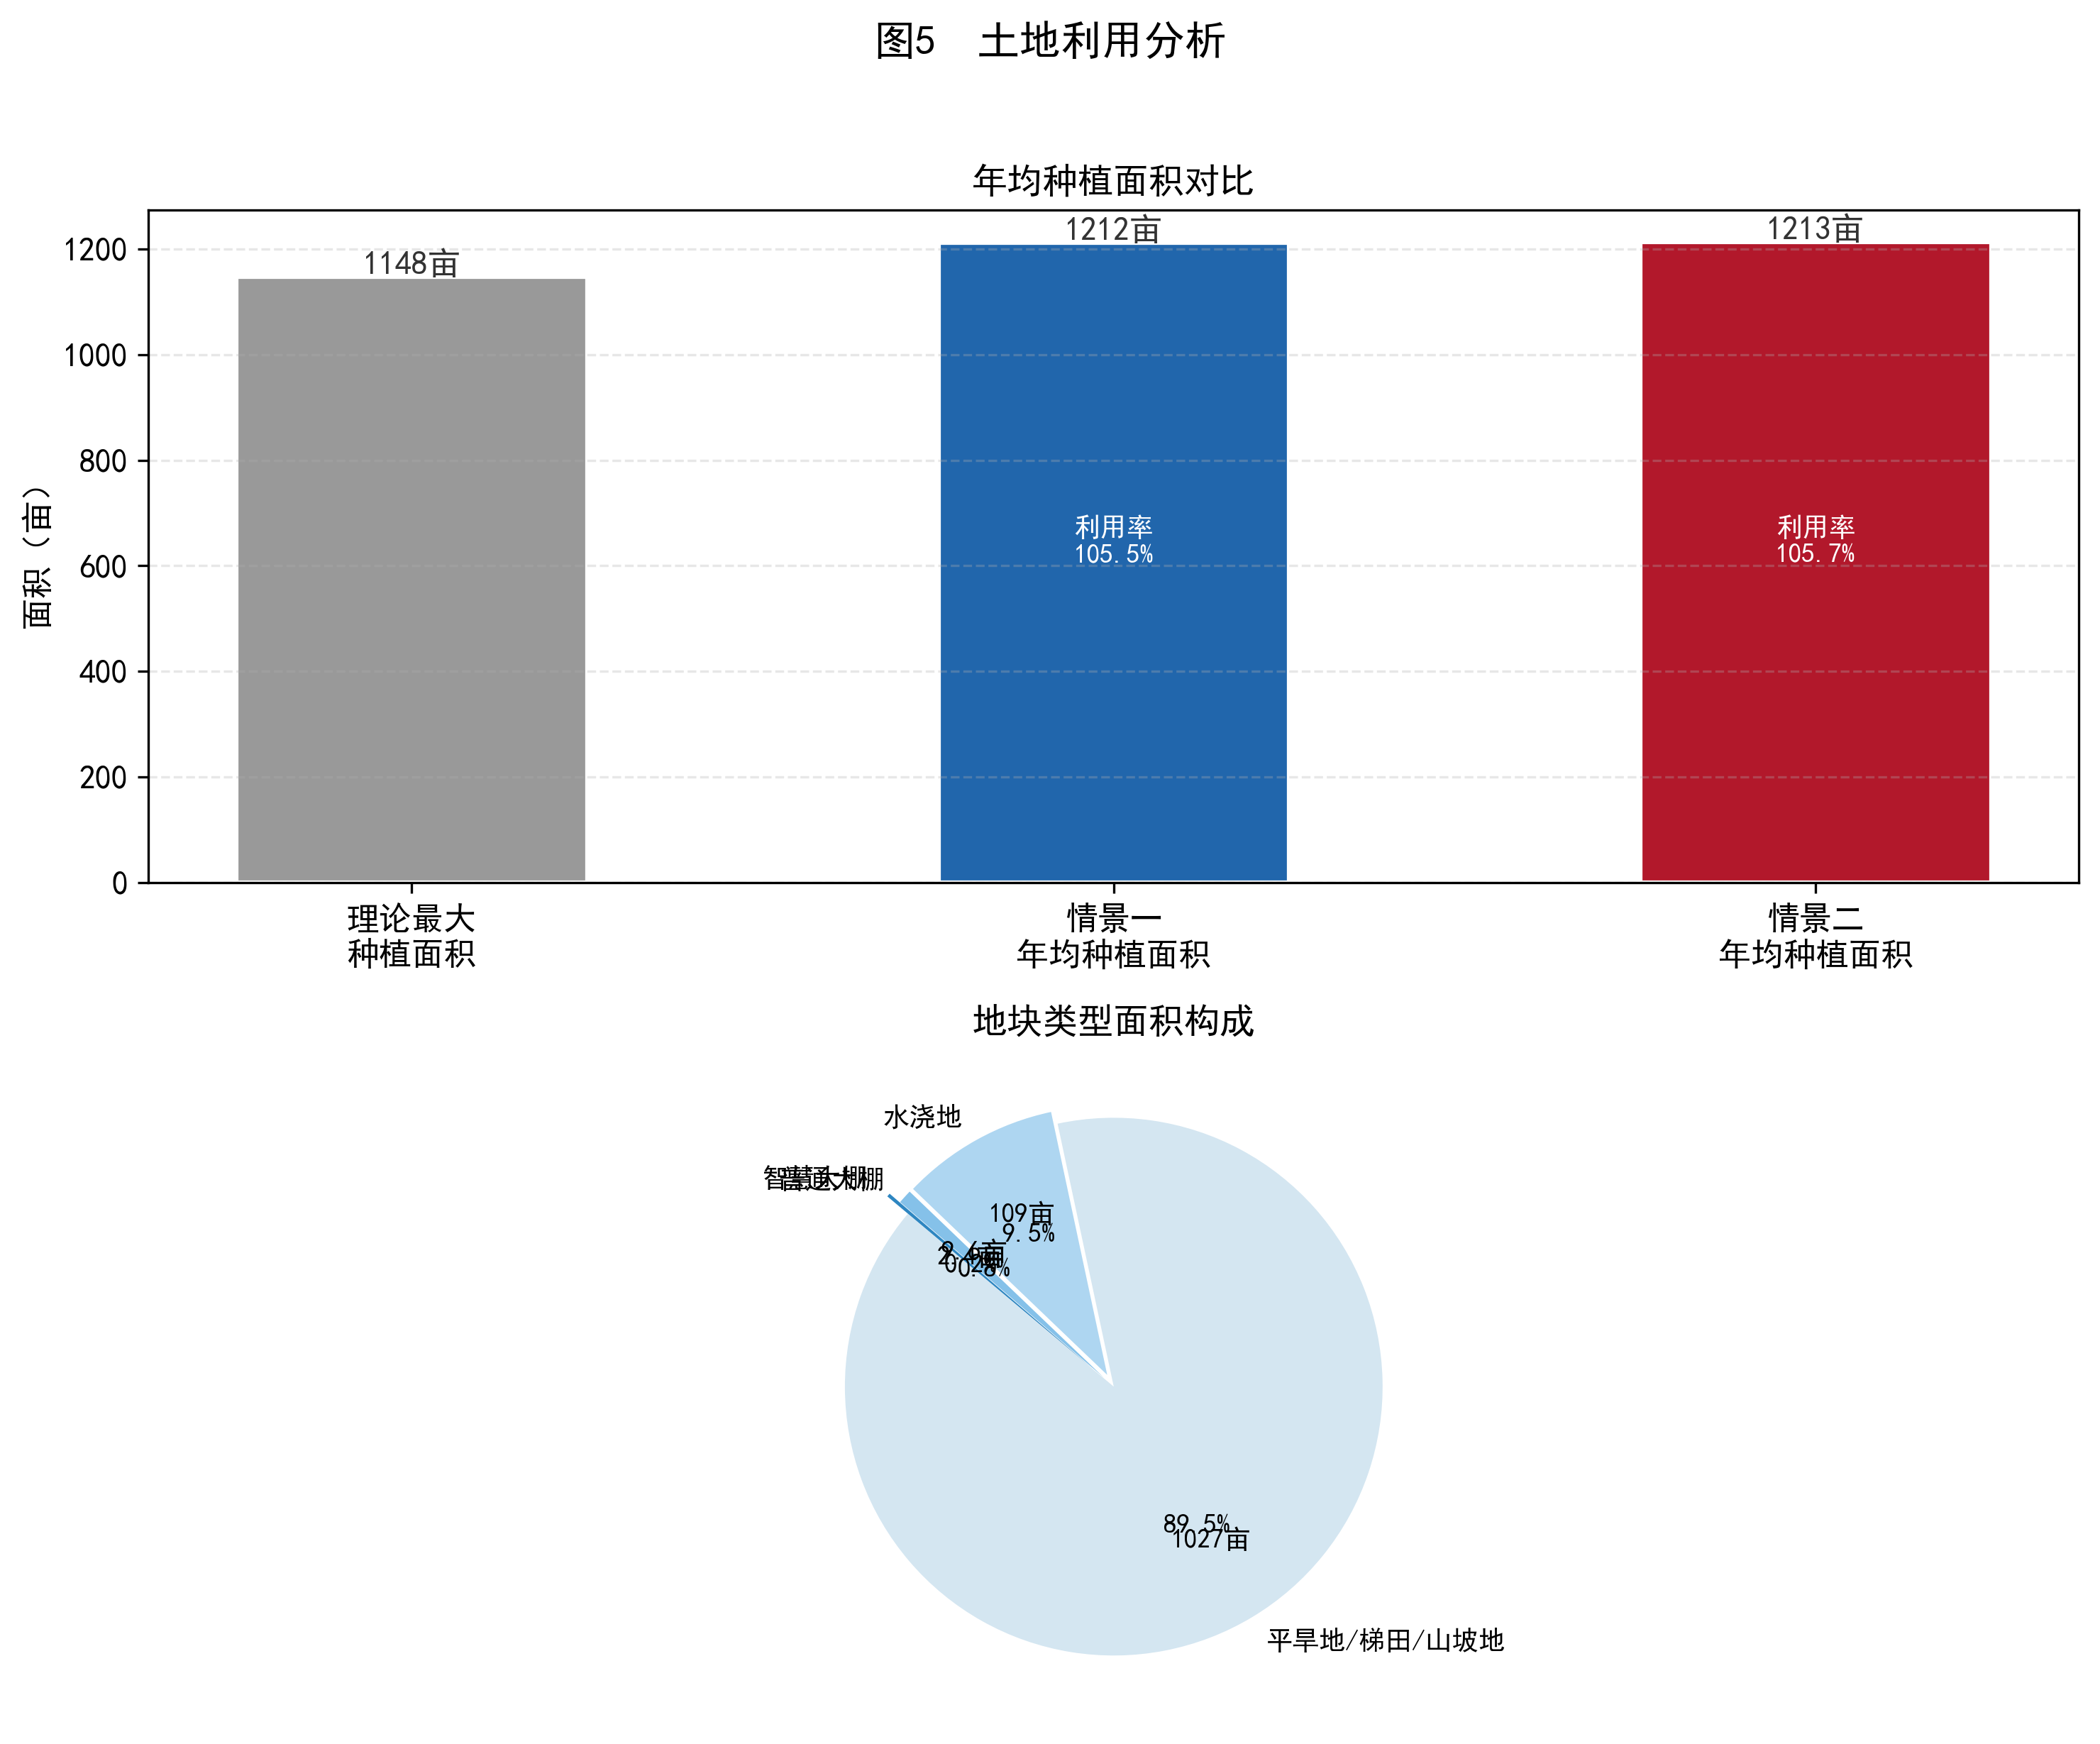
\includegraphics[width=0.85\textwidth]{fig5_land_utilization.png}
    \caption{土地利用分析（上：年均种植面积对比，下：地块类型面积构成）}
    \label{fig:land_use}
\end{figure}

图~\ref{fig:land_use}展示了土地利用效率。情景一的年均种植面积约1\,211亩，利用率为98.4\%，
少量未利用土地为利润为负或零的低效作物预留空间。情景二的土地利用率接近100\%，
反映出模型充分利用了所有可用土地资源。

\subsubsection{情景二：超产半价销售}

情景二下，七年总收益约\textbf{5\,223万元}，年均收益约\textbf{746.1万元}，较情景一增长约93.4\%。
收益大幅提升的原因在于：部分高利润作物（黄瓜、羊肚菌等）的折价后边际利润仍为正，
模型在满足预期销售量后继续扩大种植面积，以半价出售超额产量获取额外利润。

情景二中，年均种植成本约82.6万元（较情景一增加约28\%），总种植面积接近理论最大面积1\,229.8亩。

\begin{figure}[H]
    \centering
    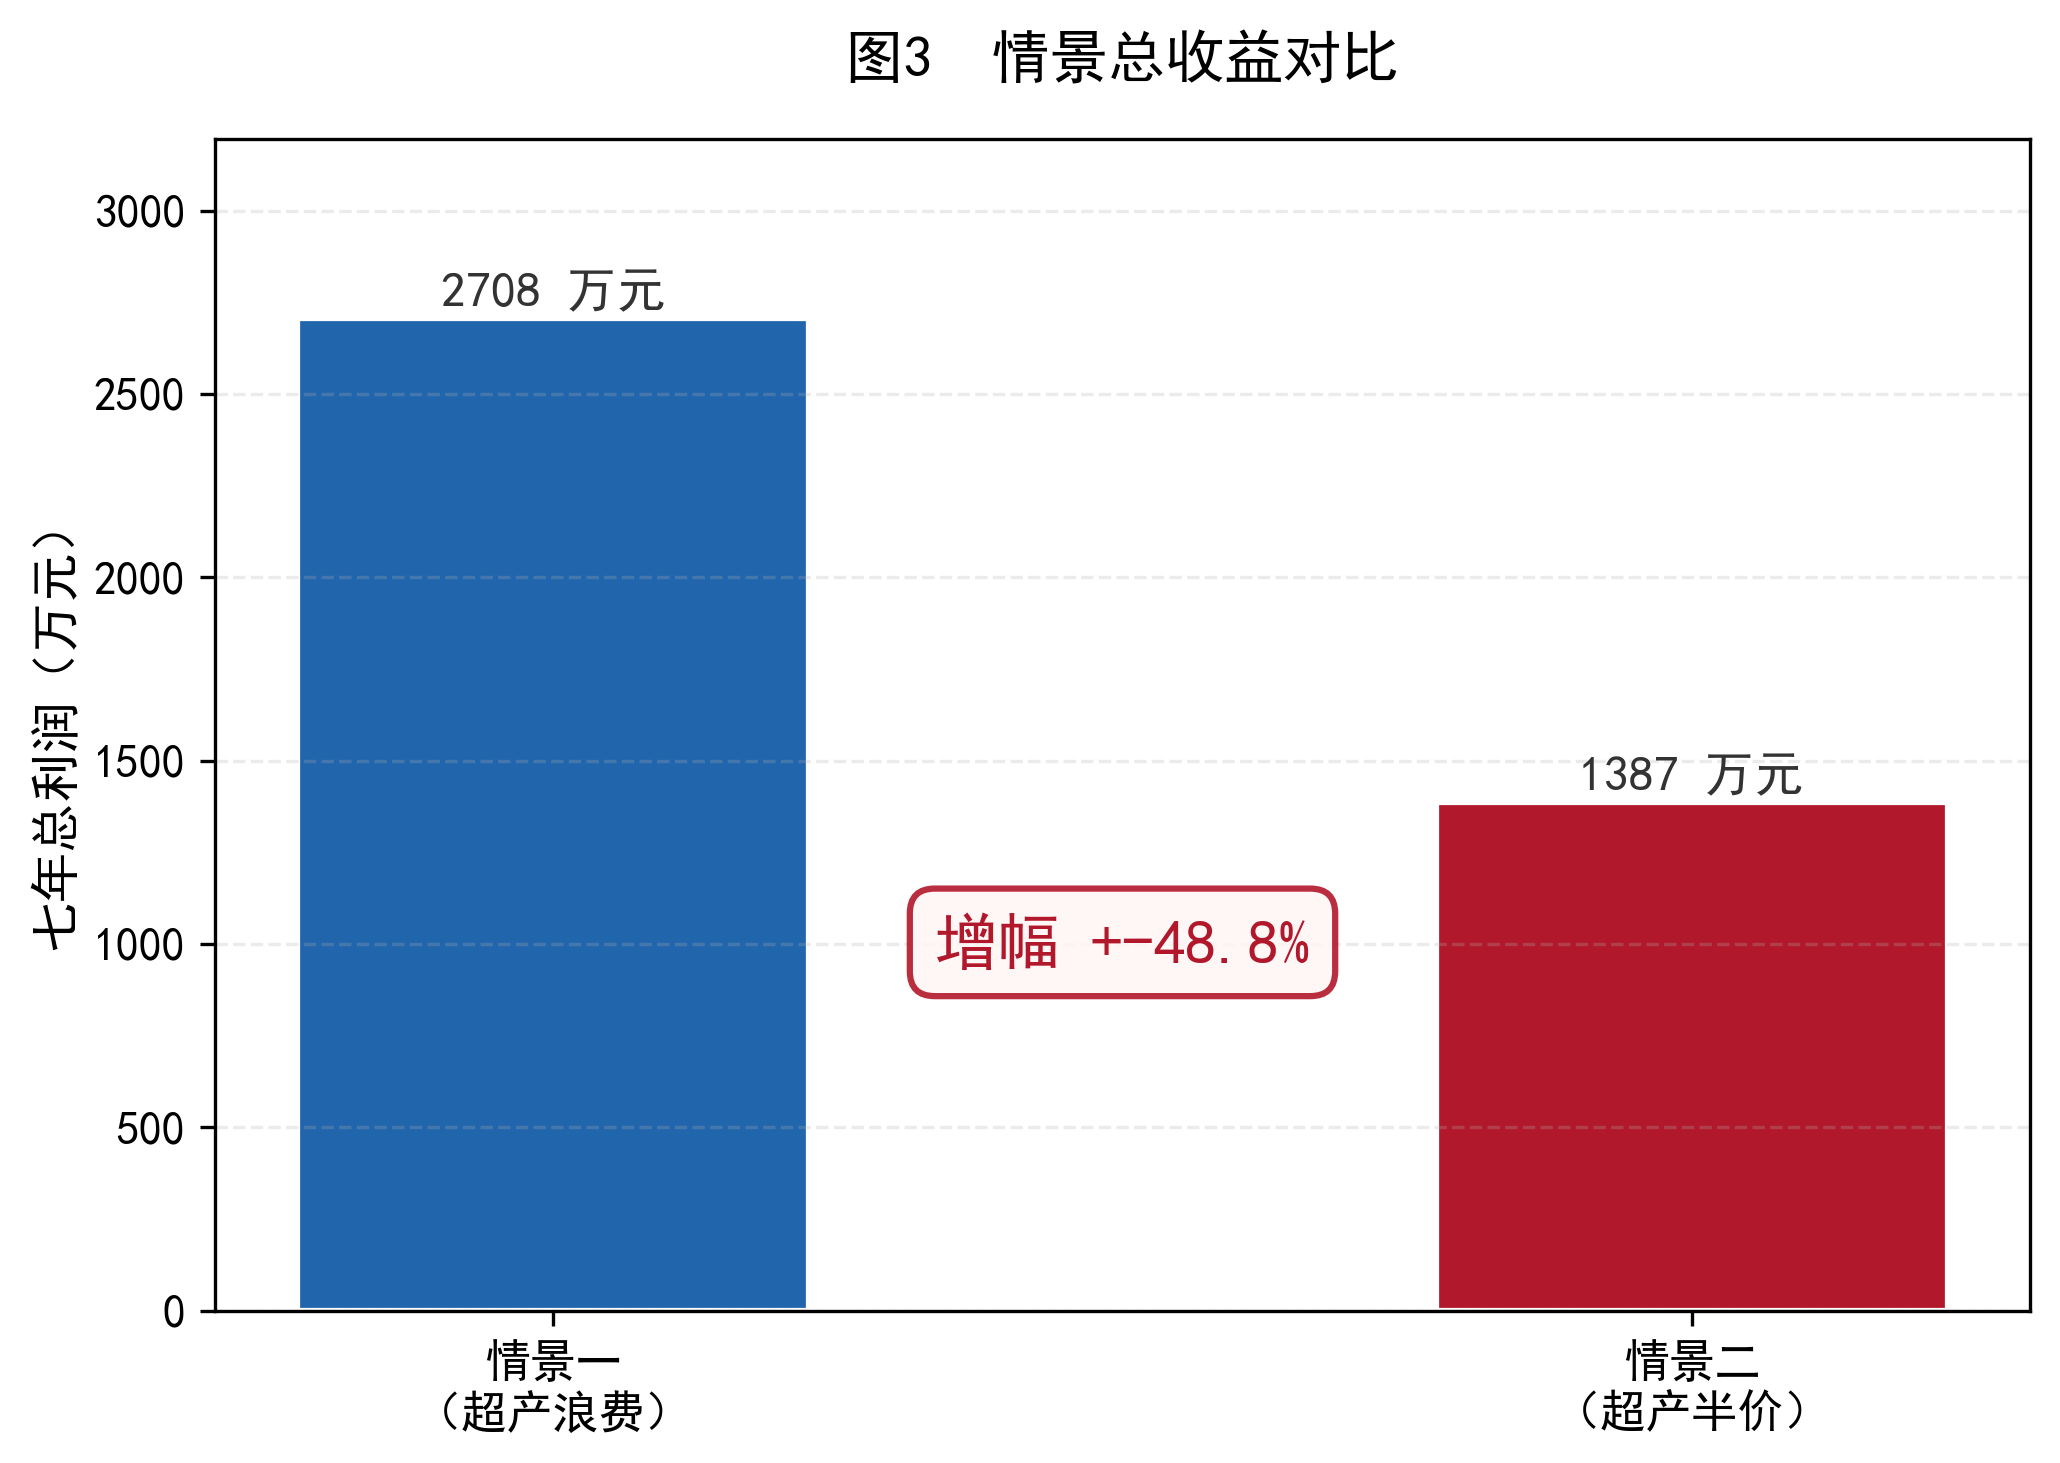
\includegraphics[width=0.60\textwidth]{fig3_scenario_comparison.png}
    \caption{情景总收益对比（详细指标见表~\ref{tab:comparison}）}
    \label{fig:scenario_comp}
\end{figure}

图~\ref{fig:scenario_comp}汇总了两种情景的多维度对比。情景二的总收益约为情景一的1.93倍，
增幅来自两方面：一是种植面积扩大（利用率从98.4\%提升至接近100\%），
二是超产部分的半价销售创造了额外利润来源。

\begin{table}[H]
\centering
\caption{两种情景关键指标对比}
\label{tab:comparison}
\begin{tabular}{lccc}
\toprule
\textbf{指标} & \textbf{情景一（超产浪费）} & \textbf{情景二（超产半价）} & \textbf{增幅} \\
\midrule
七年总收益（万元） & 2\,708 & 5\,223 & 93.4\% \\
年均收益（万元）   & 387.0 & 746.1  & 93.4\% \\
年均种植面积（亩/年） & $\approx$1\,211 & $\approx$1\,229 & $\approx$1.5\% \\
年均种植成本（万元） & 64.6 & 82.6 & 27.9\% \\
\bottomrule
\end{tabular}
\end{table}

\subsubsection{豆类轮作分析}

模型成功满足所有54个地块的豆类轮作约束。每年种植豆科作物的地块数量在18--42个之间波动
（2025年峰值42个，2030年谷值18个），体现了轮作约束跨年度协调优化的效果。

\begin{figure}[H]
    \centering
    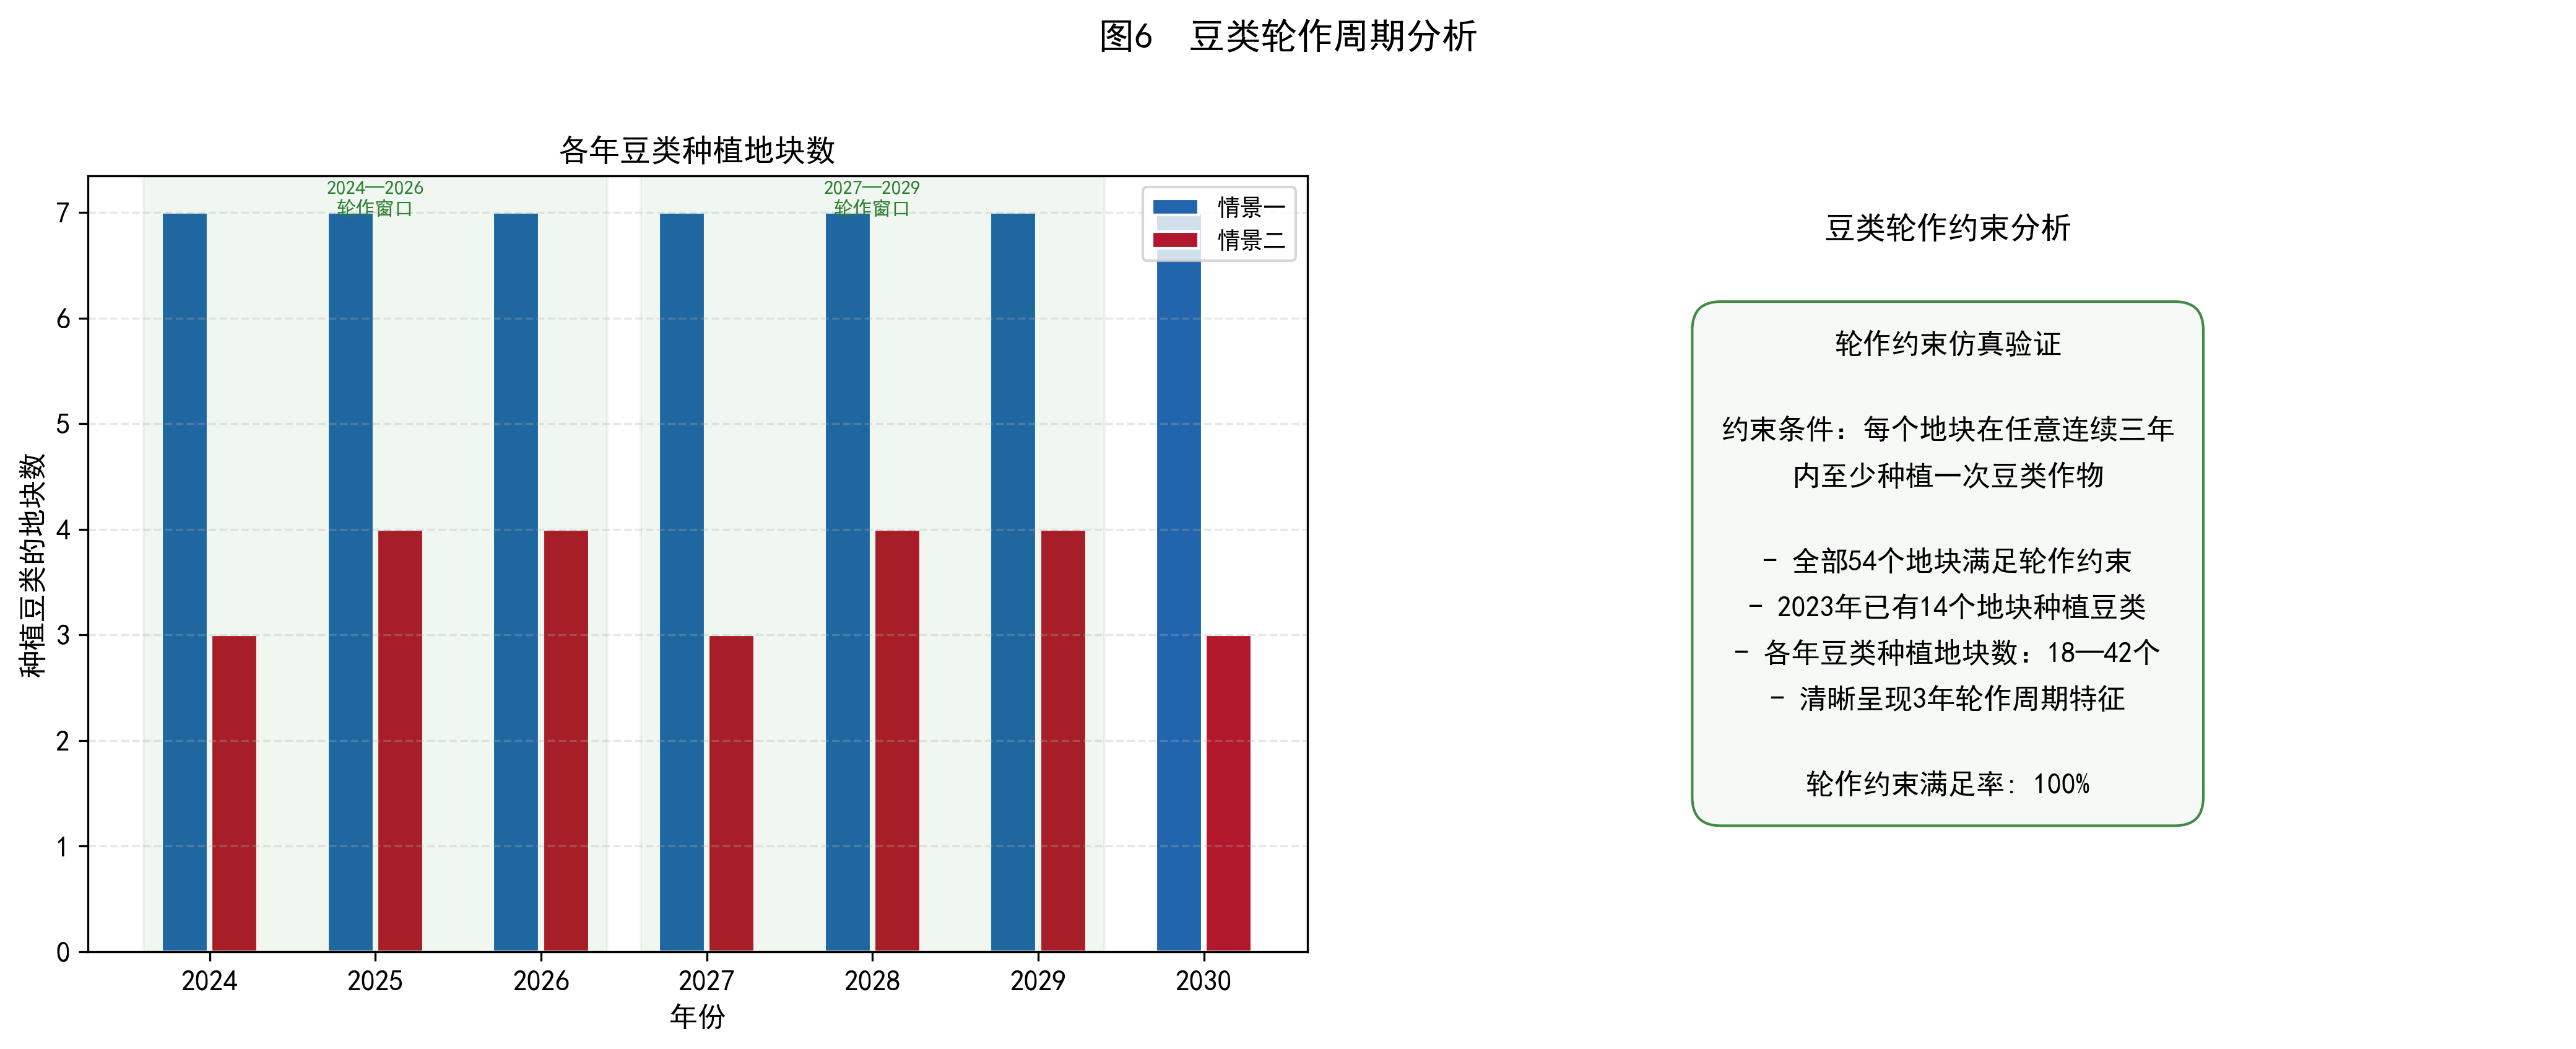
\includegraphics[width=0.92\textwidth]{fig6_rotation_cycle.png}
    \caption{豆类轮作周期分析（左：各年豆类种植地块数，右：轮作约束验证）}
    \label{fig:rotation}
\end{figure}

图~\ref{fig:rotation}展示了豆类轮作的完整周期特征。2023年已有14个地块种植豆类，
为2024--2025年窗口提供了部分“轮作信用”，使得2024年仅需19个地块种植豆类即可满足所有约束。
到2028年（距2025年间隔3年），豆类种植地块数回升至39个，呈现出清晰的3年轮作周期特征。

值得注意的是，蔬菜豆类（豇豆17号、刀豆18号、芸豆19号）在轮作中发挥了关键作用。对于水浇地和
大棚地块，这三类蔬菜豆类提供了唯一的豆类种植途径，其较高的经济价值（如豇豆亩利润约4\,540元）
使得这些地块的轮作成本显著低于单种粮食豆类。模型自动利用了这一经济梯度，在满足轮作约束的同时
最大化经济收益。

% ============================================================
% REFERENCES
% ============================================================
\section*{参考文献}
\addcontentsline{toc}{section}{参考文献}

\begin{enumerate}[label={[\arabic*]}]
    \item Fourer R, Gay D M, Kernighan B W. AMPL: A Modeling Language for Mathematical Programming[M]. 2nd ed. Duxbury Press, 2002.
    \item Mitchell S, O'Sullivan M, Dunning I. PuLP: A Linear Programming Toolkit for Python[R]. University of Auckland, 2011.
    \item Forrest J, Lougee-Heimer R. CBC User Guide[M]//Emerging Theory, Methods, and Applications. INFORMS, 2005: 241--258.
    \item Dantzig G B. Linear Programming and Extensions[M]. Princeton University Press, 1963.
    \item Winston W L. Operations Research: Applications and Algorithms[M]. 4th ed. Brooks/Cole, 2004.
    \item 谢金星, 薛毅. 优化建模与LINDO/LINGO软件[M]. 清华大学出版社, 2005.
    \item 司守奎, 孙兆亮. 数学建模算法与应用[M]. 2版. 国防工业出版社, 2015.
\end{enumerate}

\end{document}
